\chapter{Area and Volume}
\graphicspath{{foto/Chap4/}}
In this chapter have been calculated area and volume of the 3D Memory complete structure (Memory, Decoders and Sence Amplifier).

\section{Memory array}
For the area and volume evaluation of the memory, the model of \ref{fig:cube} has been used.

\begin{center}
	\begin{figure}[H]
		\centering
		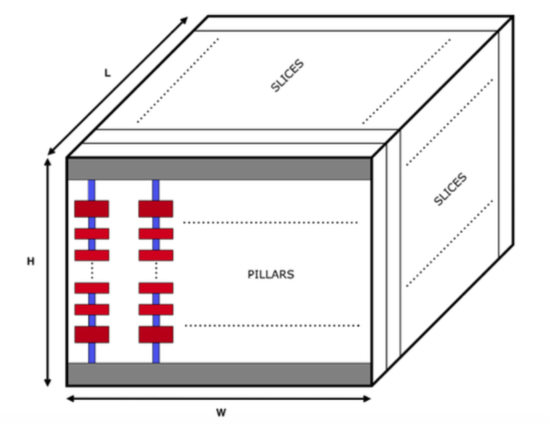
\includegraphics[scale = 0.6]{cube}
		\caption{Simplified memory structure}
		\label{fig:cube}
	\end{figure}
\end{center}

The three dimensions of the array have been computed as follows:

\begin{itemize}
	\item \textit{Width} and \textit{Length}: considering the symmetry of the model, the same pitch between two pillars in the same slice and between two pillars in two different slices has been used.
	\[
	W=N_{column} \cdot Pitch_{pp} = N_{bl} \cdot Pitch_{pp}
	\]	
	\[
	L=N_{slice} \cdot Pitch_{pp}
	\]
				
	\item \textit{Height of the stack}: the terms considered are the height of the MOS FGTs and MOS GST/SST, the pitch between contacts and GST/SST and between FGTs and GST/SST, the height of the S/D contacts, as shown in \ref{fig:pillar}.	
	\[
	H=2 \cdot Pitch_{contact-PT}+(N_{wl}-1) \cdot Pitch_{FGT-FGT}+2 \cdot Pitch_{PT-FGT}+ 2 \cdot h_{contact}
	\]

	Obviously, for planar MOS technology, $h_{contact}$ is set to zero.\\ 
	Finally, the area and the volume of the array of memory can be calculated as:
	\[
	\textbf{Memory\_Array\_Area}=H \cdot W
	\]
	\[
	\textbf{Memory\_Array\_Volume}=H \cdot W \cdot L
	\]

\begin{center}
	\begin{figure}[H]
		\centering
		\includegraphics[scale = 0.4]{section_pillars}
		\caption{Stack structure}
		\label{fig:pillar}
	\end{figure}
\end{center}
\end{itemize}

\section{Decoders}
For the area and volume evaluation of all the decoders, the model that has been used is the same described in the Chapter 2. For each decoder the number of n-type transistors was first calculated and then the number of p-type transistors; subsequently they have been multiplied by their minimum area value and then added together to calculate the total area. Finally the volume has been calculated as the multiplication of the Area and the length.

\begin{itemize}
\item{\textbf{Block Decoder}}:
The area of the \textit{Block Decoder} has been calculated as: area of the the core of the decoder added to the area of the inverter connected at the input and and at the output. In this case the number of input is given by the \textit{Block Address} while the output is equal to the number of slice $N_{slice}$. The volume is the area multiplied by the length. So:
	\[
	\#Tr\_n\_Block\_Dec = Block\_Address \cdot N_{slice} + N_{slice} + Block\_Address
	\]
	\[
	\#Tr\_p\_Block\_Dec = 2 \cdot N_{slice} + Block\_Address
	\]
	\\
	\[
	\textbf{Block\_Dec\_Area} = \#Tr\_n\_Block\_Dec \cdot Tr\_n\_Area +
	\]
	\[
	+ \#Tr\_p\_Block\_Dec \cdot Tr\_p\_Area
	\]
	\[
	\textbf{Block\_Dec\_Volume} = Block\_Dec\_Area \cdot L
	\]

\item{\textbf{Row Decoder}}:
The area of the \textit{Row Decoder} has been calculated as before but in this case the number of input is done by the \textit{Row Address} while the output is equal to the number of row that is $(N_{wl}+2)$. The volume is the area multiplied by the length. So:
	\[
	\#Tr\_n\_Row\_Dec = Row\_Address \cdot (N_{wl}+2) + (N_{wl}+2) + Row\_Address
	\]
	\[
	\#Tr\_p\_Row\_Dec = 2 \cdot (N_{wl}+2) + Row\_Address
	\]
	\\
	\[
	\textbf{Row\_Dec\_Area} = \#Tr\_n\_Row\_Dec \cdot Tr\_n\_Area +
	\]
	\[
	+ \#Tr\_p\_Row\_Dec \cdot Tr\_p\_Area
	\]
	\[
	\textbf{Row\_Dec\_Volume} = Row\_Dec\_Area \cdot L
	\]
\newpage
\item{\textbf{Column Decoder}}:
The area of the \textit{Column Decoder} has been calculated as in \textit{Row Decoder} but in this case the number of input is done by the \textit{Column Address} while the output is equal to the number of bit line that is $N_{bl}$. The volume is the area multiplied by the length. So:
	\[
	\#Tr\_n\_Column\_Dec = Column\_Address \cdot N_{bl} + N_{bl} + Column\_Address
	\]
	\[
	\#Tr\_p\_Column\_Dec = 2 \cdot N_{bl} + Column\_Address
	\]
	\\
	\[
	\textbf{Column\_Dec\_Area} = \#Tr\_n\_Column\_Dec \cdot Tr\_n\_Area + 
	\]
	\[
	+ \#Tr\_p\_Column\_Dec \cdot Tr\_p\_Area
	\]
	\[
	\textbf{Column\_Dec\_Volume} = Column\_Dec\_Area \cdot L
	\]

\item{\textbf{Decoder Address}}:
The previous variables $Block\_Address,Row\_Address,Column\_Address$ are computed as:
	\[
	Block\_Address = ceil(log2(N_{slice}))
	\]
	\[
	Row\_Address = ceil(log2(N_{wl}))
	\]
	\[
	Column\_Address = ceil(log2(\frac{N_{bl}}{N_{bit,word}}))
	\]
\end{itemize}
	
\section{Pass Transistors and Precharge Transistors}
In the total structure there are some pass transistor of n-type used to help the selection of the wanted memory cell.
\begin{itemize}
\item{\textbf{Row Pass Transistors}}:
The area has been calculated as $(N_{wl}+2)$ multiplied by the area of single transistor, while the volume is the area multiplied by the length. So:
	\[
	\textbf{Pass\_Row\_Area} = (N_{wl}+2) \cdot Tr\_n\_Area
	\]
	\[
	\textbf{Pass\_Row\_Volume} = Pass\_Row\_Area \cdot L
	\]
\item{\textbf{Column Pass Transistors}}:
The area has been calculated as $N_{bl}$ multiplied by the area of single transistor, while the volume is the area multiplied by the length. So: 
	\[
	\textbf{Pass\_Column\_Area} = N_{bl} \cdot Tr\_n\_Area
	\]
	\[
	\textbf{Pass\_Column\_Volume} = Pass\_Column\_Area \cdot L
	\]
\item{\textbf{Slice Pass Transistors}}:
The area has been calculated as $N_{bit,word}$ multiplied by the area of single transistor, while the volume is the area multiplied by the length. So:
	\[
	\textbf{Pass\_Slice\_Area} = N_{bit,word} \cdot Tr\_n\_Area
	\]
	\[
	\textbf{Pass\_Slice\_Volume} = Pass\_Slice\_Area \cdot L
	\]
\item{\textbf{Precharge Transistors}}:
The area has been calculated as $N_{bl}$ multiplied by the area of single p-type transistor, while the volume is the area multiplied by the length. So:
	\[
	\textbf{Precharge\_Area} = N_{bl} \cdot Tr\_p\_Area
	\]
	\[
	\textbf{Precharge\_Volume} = Precharge\_Area \cdot L
	\]
\end{itemize}

\section{Sense Amplifier}
The area of the \textit{Sense Amplifier} has been calculated as remembering the structure described in Chapter 2 and the volume is the area multiplied by the length. So:

	\[
	\#Tr\_n\_SA=N_{bl} \cdot 3
	\]
	\[
	\#Tr\_p\_SA=N_{bl} \cdot 3
	\]
	\\
	\[
	\textbf{SA\_Area} = \#Tr\_n\_SA \cdot Tr\_n\_Area + \#Tr\_p\_SA \cdot Tr\_p\_Area
	\]
	\[
	\textbf{SA\_Volume} = SA\_Area \cdot L
	\]

\section{Total Area and Total Volume}
The total area has been calculated has the sum of the area of the memory array and all the boundary circuits:
	\[
	\textbf{Total\_Area}= Memory\_Array\_Area + Block\_Dec\_Area + Row\_Dec\_Area + 
	\]
	\[
	+Column\_Dec\_Area + Pass\_Row\_Area + Pass\_Column\_Area + 
	\]
	\[
	Pass\_Slice\_Area +  SA\_Area
	\]
The total volume has been calculated has the sum of the volume of the memory array and all the boundary circuits:
	\[
	\textbf{Total\_Volume}= Memory\_Array\_Volume + Block\_Dec\_Volume + Row\_Dec\_Volume + 
	\]
	\[
	+Column\_Dec\_Volume + Pass\_Row\_Volume + Pass\_Column\_Volume + 
	\]
	\[
	Pass\_Slice\_Volume +  SA\_Volume
	\]

\section{Simulation result}
In order to verify the the computations made before, it has been made a simulation; in particular it has been reported four graph in which are represented how the area and the volume change with the value of $N_{wl}$ and $N_{bl}$ and with the value of $N_{slice}$. In particular, the array of values it has been considered for both $N_{wl}$ and $N_{bl}$ is $[64, 128, 256, 512, 1024, 2048]$ while for $N_{slice}$ is $[32, 64, 128, 256]$. For each simulation point, it has been assumed that $N_{bl}=N_{wl}$, because usually the memory arrays are made as square as possible, for reasons of space availability on the board.
\\The behaviours represented are reasonable: in the first two graphs \ref{fig:1} and \ref{fig:2} there is a square dependency $N_{wl}$ and $N_{bl}$. Changing the value of these parameters, the total area and volume increase of one order of magnitude in the bigger case (2048x2048) respect to the the smaller one (64x64), with a maximum values of $2\cdot10^{-7}m^{2}$ for the Total Area and $6\cdot10^{-14}m^{3}$ for the Total Volume.
In the other two graphs \ref{fig:3} and \ref{fig:4} there is a linear dependency $N_{slice}$. Changing the value of this parameter, the total area not increase significantly, while the volume increase of one order of magnitude. The maximum values are $5.21\cdot10^{-8}m^{2}$ for the Total Area and $4\cdot10^{-12}m^{3}$ for the Total Volume.
\\The results obtained are reported in the figures below.

\begin{center}
	\begin{figure}[H]
		\centering
		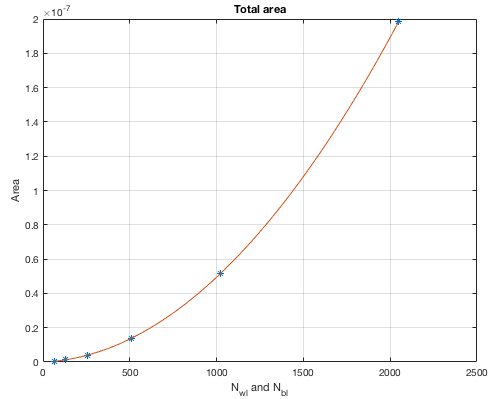
\includegraphics[scale=0.6]{Area_Nwl_Nbl.png}
		\caption{Simulation of the Total Area value, varying the size of the memory array} 
		\label{fig:1}
	\end{figure}
\end{center}

\begin{center}
	\begin{figure}[H]
		\centering
		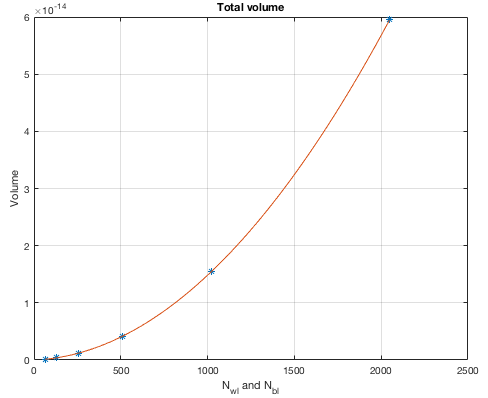
\includegraphics[scale=0.6]{Volume_Nwl_Nbl.png}
		\caption{Simulation of the Total Volume value, varying the size of the memory array}
		\label{fig:2} 
	\end{figure}
\end{center}

\begin{center}
	\begin{figure}[H]
		\centering
		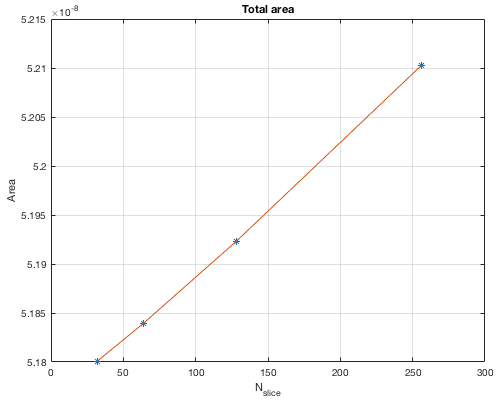
\includegraphics[scale=0.6]{Area_Nslice.png}
		\caption{Simulation of the Total Area value, varying the number of slice} 
		\label{fig:3}
	\end{figure}
\end{center}

\begin{center}
	\begin{figure}[H]
		\centering
		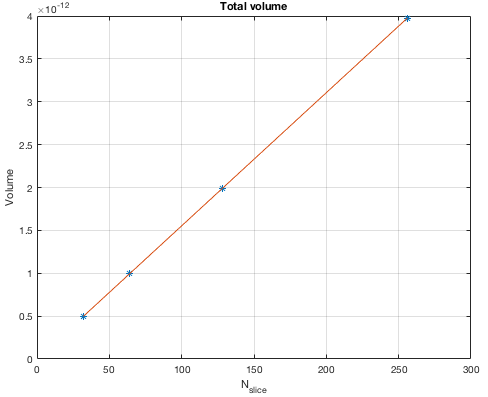
\includegraphics[scale=0.6]{Volume_Nslice.png}
		\caption{Simulation of the Total Volume value, varying the number of slice} 
		\label{fig:4}
	\end{figure}
\end{center}
